\documentclass{standalone}
\usepackage{tikz}
\usetikzlibrary{patterns, positioning}

\begin{document}
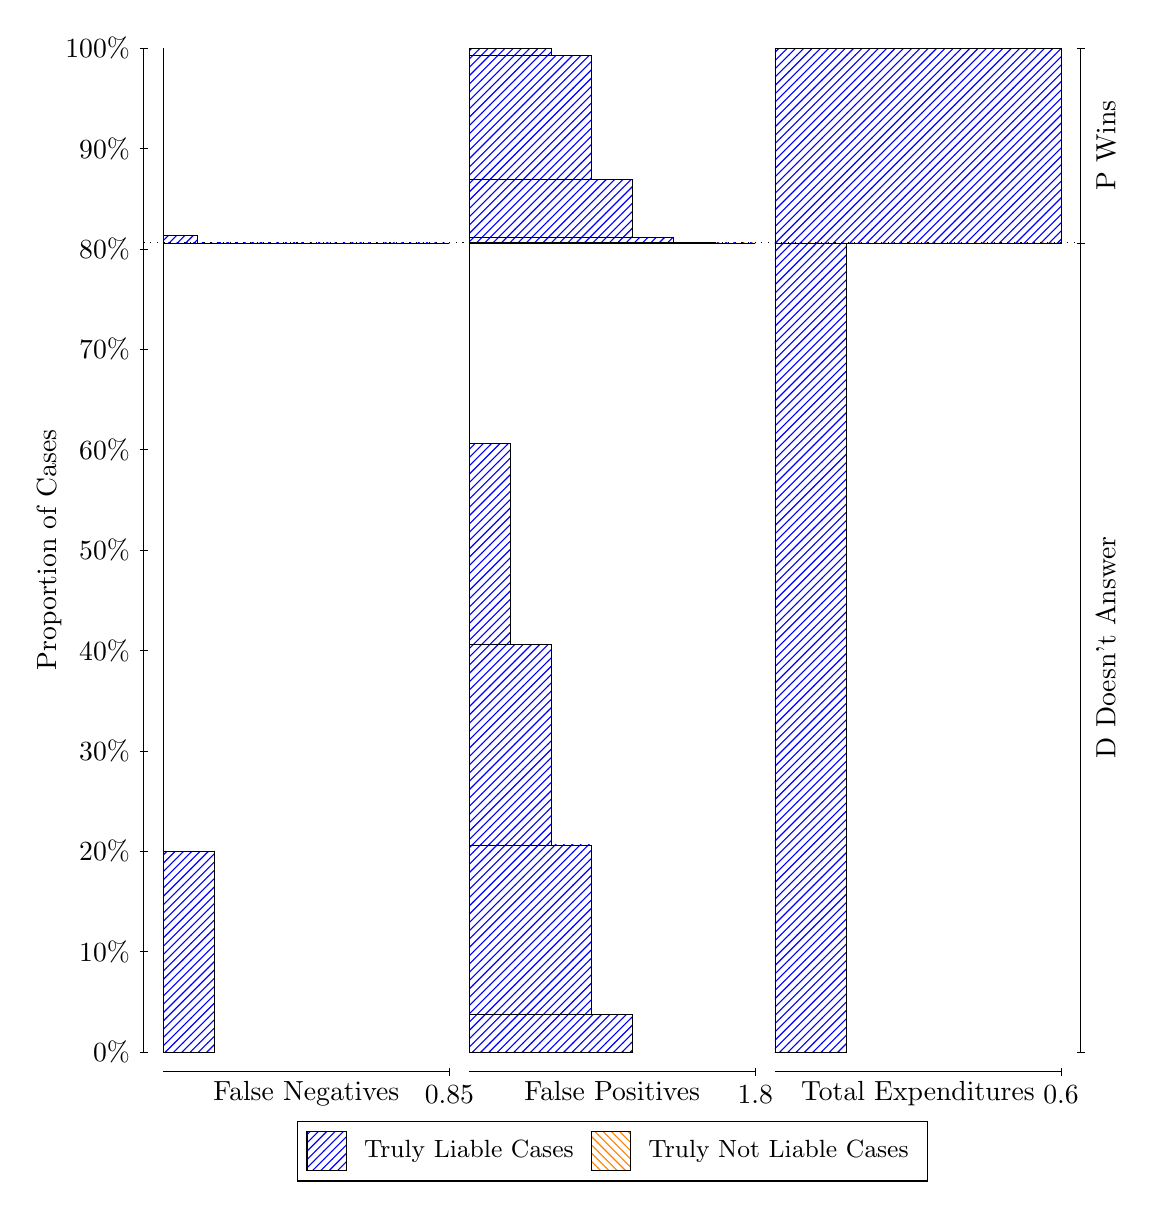
\begin{tikzpicture}
\draw[black, very thin] (1.5,1.75) -- (1.5,14.5);
\node[rotate=90, anchor=center] at (0.3, 8.125) {Proportion of Cases};
\draw[black, very thin] (1.45,1.75) -- (1.55,1.75);
\node[anchor=east] at (1.45, 1.75) {0\%};
\draw[black, very thin] (1.45,3.025) -- (1.55,3.025);
\node[anchor=east] at (1.45, 3.025) {10\%};
\draw[black, very thin] (1.45,4.3) -- (1.55,4.3);
\node[anchor=east] at (1.45, 4.3) {20\%};
\draw[black, very thin] (1.45,5.575) -- (1.55,5.575);
\node[anchor=east] at (1.45, 5.575) {30\%};
\draw[black, very thin] (1.45,6.85) -- (1.55,6.85);
\node[anchor=east] at (1.45, 6.85) {40\%};
\draw[black, very thin] (1.45,8.125) -- (1.55,8.125);
\node[anchor=east] at (1.45, 8.125) {50\%};
\draw[black, very thin] (1.45,9.4) -- (1.55,9.4);
\node[anchor=east] at (1.45, 9.4) {60\%};
\draw[black, very thin] (1.45,10.675) -- (1.55,10.675);
\node[anchor=east] at (1.45, 10.675) {70\%};
\draw[black, very thin] (1.45,11.95) -- (1.55,11.95);
\node[anchor=east] at (1.45, 11.95) {80\%};
\draw[black, very thin] (1.45,13.225) -- (1.55,13.225);
\node[anchor=east] at (1.45, 13.225) {90\%};
\draw[black, very thin] (1.45,14.5) -- (1.55,14.5);
\node[anchor=east] at (1.45, 14.5) {100\%};

\draw[black, very thin] (13.4,1.75) -- (13.4,14.5);
\draw[black, very thin] (13.35,1.75) -- (13.45,1.75);
\node[anchor=west] at (13.35, 1.75) {};
\draw[black, very thin] (13.35,12.026) -- (13.45,12.026);
\node[anchor=west] at (13.35, 12.026) {};
\draw[black, very thin] (13.35,14.5) -- (13.45,14.5);
\node[anchor=west] at (13.35, 14.5) {};

\draw[black, very thin, pattern color=blue, pattern=north east lines] (1.75,1.75) rectangle (2.3912,4.2999);
\draw[black, very thin, pattern color=orange, pattern=north west lines] (1.75,4.2999) rectangle (1.75,4.2999);
\draw[black, very thin, pattern color=blue, pattern=north east lines] (1.75,4.2999) rectangle (1.75,12.026);
\draw[black, very thin, pattern color=blue, pattern=north east lines] (1.75,12.026) rectangle (5.3833,12.026);
\draw[black, very thin, pattern color=blue, pattern=north east lines] (1.75,12.026) rectangle (4.3147,12.026);
\draw[black, very thin, pattern color=blue, pattern=north east lines] (1.75,12.026) rectangle (3.2461,12.026);
\draw[black, very thin, pattern color=blue, pattern=north east lines] (1.75,12.026) rectangle (3.2461,12.026);
\draw[black, very thin, pattern color=blue, pattern=north east lines] (1.75,12.026) rectangle (2.1775,12.026);
\draw[black, very thin, pattern color=blue, pattern=north east lines] (1.75,12.026) rectangle (2.1775,12.121);
\draw[black, very thin, pattern color=orange, pattern=north west lines] (1.75,12.121) rectangle (1.75,12.121);
\draw[black, very thin, pattern color=blue, pattern=north east lines] (1.75,12.121) rectangle (1.75,14.5);
\draw[black, very thin, pattern color=orange, pattern=north west lines] (5.6333,1.75) rectangle (7.7095,1.75);
\draw[black, very thin, pattern color=blue, pattern=north east lines] (5.6333,1.75) rectangle (7.7095,2.2309);
\draw[black, very thin, pattern color=blue, pattern=north east lines] (5.6333,2.2309) rectangle (7.1905,4.3792);
\draw[black, very thin, pattern color=blue, pattern=north east lines] (5.6333,4.3792) rectangle (6.6714,6.9258);
\draw[black, very thin, pattern color=blue, pattern=north east lines] (5.6333,6.9258) rectangle (6.1524,9.4758);
\draw[black, very thin, pattern color=blue, pattern=north east lines] (5.6333,9.4758) rectangle (5.6333,12.026);
\draw[black, very thin, pattern color=orange, pattern=north west lines] (5.6333,12.026) rectangle (9.2667,12.026);
\draw[black, very thin, pattern color=blue, pattern=north east lines] (5.6333,12.026) rectangle (9.2667,12.026);
\draw[black, very thin, pattern color=orange, pattern=north west lines] (5.6333,12.026) rectangle (8.7476,12.026);
\draw[black, very thin, pattern color=blue, pattern=north east lines] (5.6333,12.026) rectangle (8.7476,12.027);
\draw[black, very thin, pattern color=orange, pattern=north west lines] (5.6333,12.027) rectangle (8.2286,12.027);
\draw[black, very thin, pattern color=blue, pattern=north east lines] (5.6333,12.027) rectangle (8.2286,12.098);
\draw[black, very thin, pattern color=orange, pattern=north west lines] (5.6333,12.098) rectangle (7.7095,12.098);
\draw[black, very thin, pattern color=blue, pattern=north east lines] (5.6333,12.098) rectangle (7.7095,12.829);
\draw[black, very thin, pattern color=orange, pattern=north west lines] (5.6333,12.829) rectangle (7.1905,12.829);
\draw[black, very thin, pattern color=blue, pattern=north east lines] (5.6333,12.829) rectangle (7.1905,14.405);
\draw[black, very thin, pattern color=blue, pattern=north east lines] (5.6333,14.405) rectangle (6.6714,14.5);
\draw[black, very thin, pattern color=blue, pattern=north east lines] (5.6333,14.5) rectangle (6.1524,14.5);
\draw[black, very thin, pattern color=blue, pattern=north east lines] (5.6333,14.5) rectangle (5.6333,14.5);
\draw[black, very thin, pattern color=orange, pattern=north west lines] (9.5167,1.75) rectangle (10.425,1.75);
\draw[black, very thin, pattern color=blue, pattern=north east lines] (9.5167,1.75) rectangle (10.425,12.026);
\draw[black, very thin, pattern color=orange, pattern=north west lines] (9.5167,12.026) rectangle (13.15,12.026);
\draw[black, very thin, pattern color=blue, pattern=north east lines] (9.5167,12.026) rectangle (13.15,14.5);
\draw[black, dotted] (1.5,12.026) -- (13.4,12.026);
\draw[black, very thin] (1.75,1.5) -- (5.3833,1.5);
\node[anchor=north] at (3.5667, 1.5) {False Negatives};
\draw[black, very thin] (5.3833,1.45) -- (5.3833,1.55);
\node[anchor=north] at (5.3833, 1.45) {0.85};

\draw[black, very thin] (5.6333,1.5) -- (9.2667,1.5);
\node[anchor=north] at (7.45, 1.5) {False Positives};
\draw[black, very thin] (9.2667,1.45) -- (9.2667,1.55);
\node[anchor=north] at (9.2667, 1.45) {1.8};

\draw[black, very thin] (9.5167,1.5) -- (13.15,1.5);
\node[anchor=north] at (11.333, 1.5) {Total Expenditures};
\draw[black, very thin] (13.15,1.45) -- (13.15,1.55);
\node[anchor=north] at (13.15, 1.45) {0.6};

\node[black, centered, rotate=90] at (13.72, 6.8879) {D Doesn't Answer};
\node[black, centered, rotate=90] at (13.72, 13.263) {P Wins};

\draw (7.449999999999999,1.5) node[draw=none] (baseCoordinate) {};
\begin{scope}[align=center]
        \matrix[scale=0.5, draw=black, below=0.5cm of baseCoordinate, nodes={draw}, column sep=0.1cm]{
            \node[rectangle, draw, minimum width=0.5cm, minimum height=0.5cm, pattern=north east lines, pattern color=blue] {}; &
            \node[draw=none, font=\small] (B) {Truly Liable Cases}; &
            \node[rectangle, draw, minimum width=0.5cm, minimum height=0.5cm, pattern=north west lines, pattern color=orange] {}; &
            \node[draw=none, font=\small] (B) {Truly Not Liable Cases}; \\
            };
\end{scope}

\end{tikzpicture}
\end{document}